\documentclass[11pt]{article}
\usepackage[margin=1in]{geometry} 
\usepackage{amsmath,amsthm,amssymb}
\usepackage{enumitem, graphicx, float, caption}
\usepackage{amsmath}
\usepackage{bm}
\usepackage{parskip}
\usepackage{lipsum}
\usepackage{tikz}
\usepackage{listings}
\usepackage{xcolor}
\usepackage[utf8]{inputenc}
\usetikzlibrary{arrows.meta}

\definecolor{codegreen}{rgb}{0,0.6,0}
\definecolor{codegray}{rgb}{0.5,0.5,0.5}
\definecolor{codepurple}{rgb}{0.58,0,0.82}
\definecolor{backcolour}{rgb}{0.95,0.95,0.92}

\lstdefinestyle{mystyle}{
    backgroundcolor=\color{backcolour},   
    commentstyle=\color{codegreen},
    keywordstyle=\color{magenta},
    numberstyle=\tiny\color{codegray},
    stringstyle=\color{codepurple},
    basicstyle=\ttfamily\tiny,
    breakatwhitespace=false,         
    breaklines=true,                 
    captionpos=b,                    
    keepspaces=true,                 
    numbers=left,                    
    numbersep=5pt,                  
    showspaces=false,                
    showstringspaces=false,
    showtabs=false,                  
    tabsize=2
}

\lstset{xleftmargin=.020\textwidth, xrightmargin=.020\textwidth}

\setcounter{MaxMatrixCols}{26}
\setlength\parindent{0pt}

\begin{document}
\title{Midterm 1}

\author{Nathan Burwig \\ MATH 87 Math Modeling} 
\maketitle
%%%%%%%%%%%%%%%%%%%%%%%%%%%%%%%%%%%%%%%%%%%%%%%%%%%%%%%%%%%%%%%%%

    This is the midterm report of Nathan Burwig for the Fall Semester of 2022
    
    \section{The problem}
        We are given the problem of minimzing the costs of a certain (rubber) duck
        shipping and manufacturing company. What follows is my attempt to do
        so, along with a few other optimization problems related to this one

        \subsection{Section 1}

        We start this section, with a clearly labled network-flow model.
        Primarily, this section features the actual graph I will be using to
        model this network flow problem. Each node represents a major city
        where ducks are freighted between. The number associated with each edge
        is the price per duck in dollars that it costs to ship along that
        route. We have a source and terminal node to help process some of the
        data involved. \\

    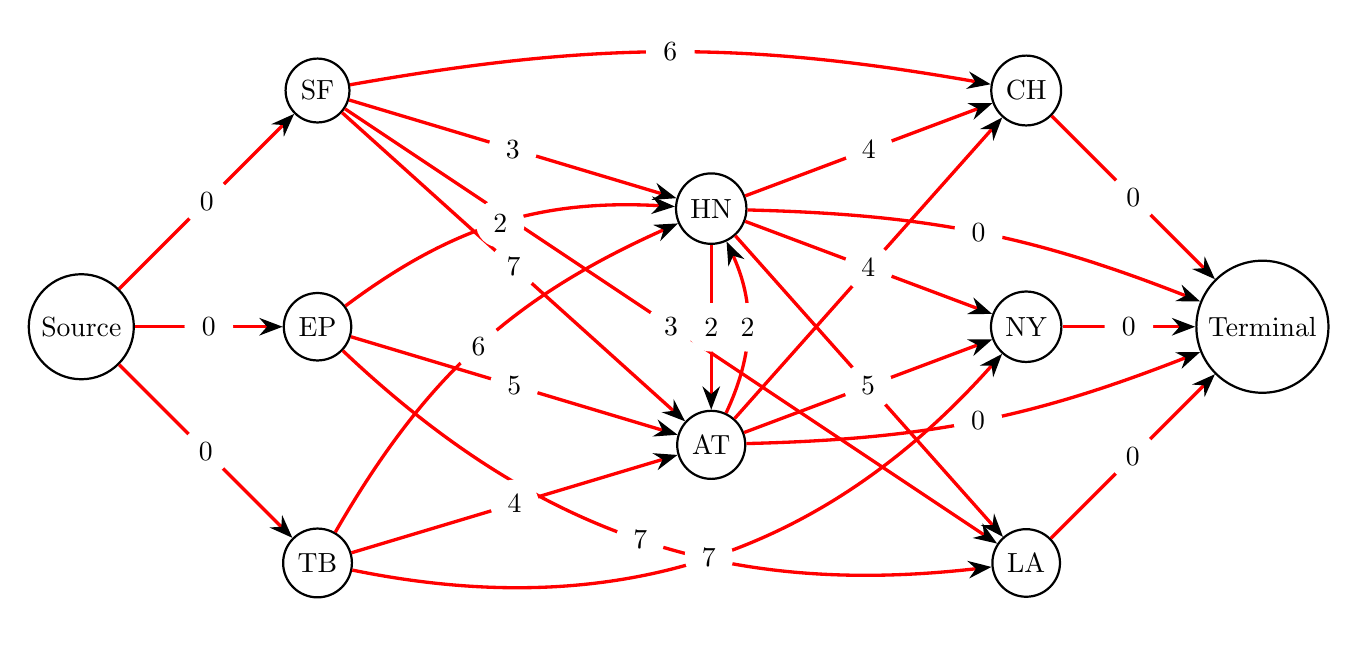
\begin{tikzpicture}
        \begin{scope}[every node/.style = {circle, thick, draw}]
            \node (A) at (0, 1)   {Source};

            \node (B) at (3, 4)   {SF};
            \node (C) at (3, 1)   {EP};
            \node (D) at (3,-2)   {TB};

            \node (E) at (8,  2.5)   {HN};
            \node (F) at (8, -0.5)   {AT};

            \node (G) at (12, 4)  {CH};
            \node (H) at (12, 1)  {NY};
            \node (I) at (12,-2)  {LA};

            \node (J) at (15, 1)  {Terminal};
        \end{scope}

        \begin{scope}[>={Stealth[black]},
                        every node/.style={fill=white,circle},
                        every edge/.style={draw=red,very thick}]
            \path [->] (A) edge node {$0$} (B);
            \path [->] (A) edge node {$0$} (C);
            \path [->] (A) edge node {$0$} (D);

            \path [->] (B) edge[bend left=10] node {$6$} (G);
            \path [->] (B) edge node {$3$} (I);
            \path [->] (B) edge node {$3$} (E);
            \path [->] (B) edge node {$7$} (F);

            \path [->] (C) edge[bend left=20] node {$2$} (E);
            \path [->] (C) edge[bend right=25] node {$7$} (I);
            \path [->] (C) edge node {$5$} (F);

            \path [->] (D) edge[bend right=30] node {$7$} (H);
            \path [->] (D) edge[bend left=18] node {$6$} (E);
            \path [->] (D) edge node {$4$} (F);

            \path [->] (E) edge node {$4$} (G);
            \path [->] (E) edge node {$5$} (I);
            \path [->] (E) edge node {$6$} (H);
            \path [->] (E) edge node {$2$} (F);
            \path [->] (E) edge[bend left=10] node {$0$} (J);
            
            \path [->] (F) edge node {$4$} (G);
            \path [->] (F) edge node {$5$} (H);
            \path [->] (F) edge[bend right=25] node {$2$} (E);
            \path [->] (F) edge[bend right=10] node {$0$} (J);

            \path [->] (G) edge node {$0$} (J);
            \path [->] (H) edge node {$0$} (J);
            \path [->] (I) edge node {$0$} (J);

        \end{scope}
    \end{tikzpicture}

    Note that the source and terminal nodes have no costs associated with them,
    as these notes are somewhat of a dummy variable. The Source node could
    represent something like a manufacturing facility, and the Terminal node
    would be the actual customers who recieve the ducks.

    There are also a handful of constraints that we have to consider given this
    problem. We know that no single route (edge) can have more than 200 ducks go over
    it. We also know that there are specific demands for each node. These
    demans are not shown in the above diagram, simply because the diagram would
    become too chaotic. If we know we don't want to send any more than a given
    cities demand, though, (as we don't want to have ducks shipped that don't
    sell) then we know the demand can be express in the following inequality
    constraints.
        \begin{align*}
            \centering
            \text{Source}           &\leq 0    \\  
            \text{Santa Fe  (SF)}   &\leq -700 \\
            \text{El Paso   (EP)}   &\leq -200 \\
            \text{Tampa Bay (TB)}   &\leq -200 \\
            \text{Chicago   (CH)}   &\leq 200 \\
            \text{LA        (LA)}   &\leq 200 \\
            \text{NY        (NY)}   &\leq 250 \\
            \text{Houston   (HN)}   &\leq 300 \\
            \text{Atlanta   (AT)}   &\leq 150 \\
            \text{Terminal}         &\leq 0   
        \end{align*}
   We assign a negative value to the constraints of the warehouse cities as
   they need to get rid of ducks that are stored, and we have 0's on the source
   and terminal as, in this context, the ducks going through them is not of
   significance to the total system.

   \subsection{Formulating the Linear Program}
   
    We know that we want to minimize the costs associated with shipping ducks,
    or to find the best way to ship the ducks with the minimum cost
    associated. To do this, we want to find some set of constraints that gives
    us the conservation quantities for our system of nodes. In this case, we
    know that (because we have a terminal and source node) anything that goes
    into a node, must come out of the node, unless it is terminal or source. We
    can use this to write a set of constraint equations that will form our
    constraint matrix A. In order to do this, though, we will want there to be
    a mapping between some useful variables (ie $e_i$) and the edge between two
    cities. The mapping will go as follows...
    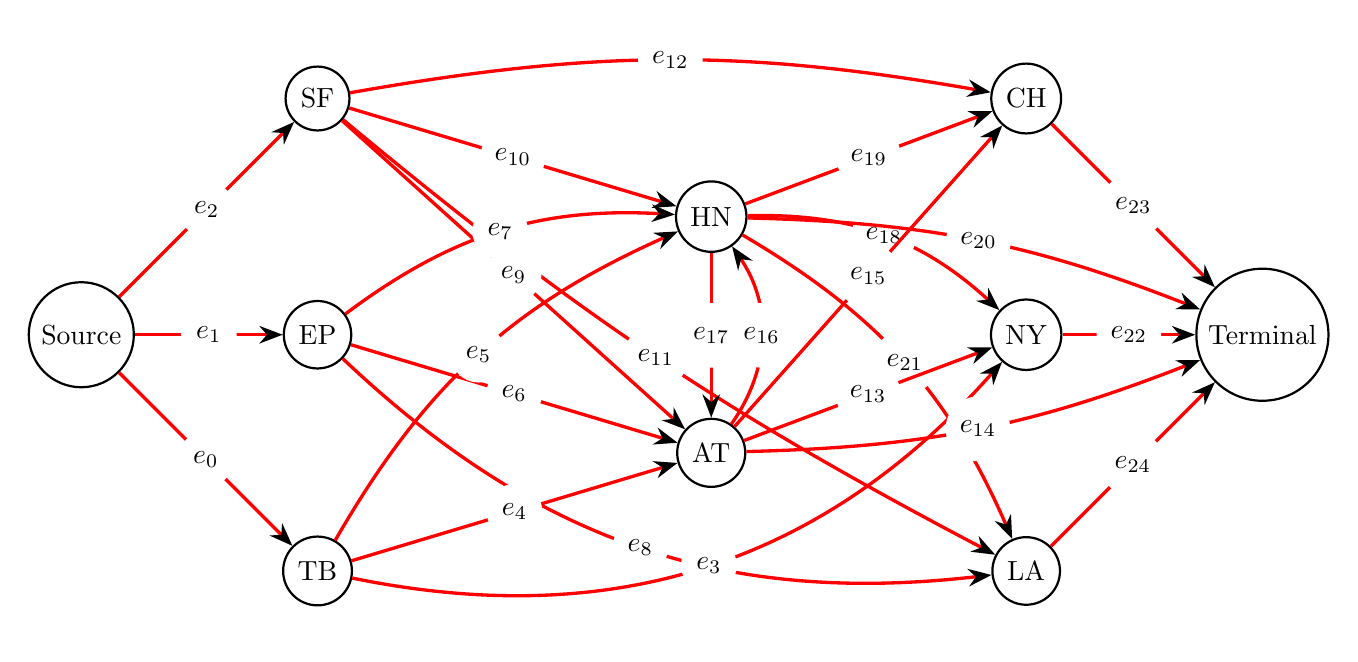
\begin{tikzpicture}
        \begin{scope}[every node/.style = {circle, thick, draw}]
            \node (A) at (0, 1)   {Source};

            \node (B) at (3, 4)   {SF};
            \node (C) at (3, 1)   {EP};
            \node (D) at (3,-2)   {TB};

            \node (E) at (8,  2.5)   {HN};
            \node (F) at (8, -0.5)   {AT};

            \node (G) at (12, 4)  {CH};
            \node (H) at (12, 1)  {NY};
            \node (I) at (12,-2)  {LA};

            \node (J) at (15, 1)  {Terminal};
        \end{scope}

        \begin{scope}[>={Stealth[black]},
                        every node/.style={fill=white,circle},
                        every edge/.style={draw=red,very thick}]
            \path [->] (A) edge node {$e_2$} (B);
            \path [->] (A) edge node {$e_1$} (C);
            \path [->] (A) edge node {$e_0$} (D);

            \path [->] (B) edge[bend left=10] node {$e_{12}$} (G);
            \path [->] (B) edge[bend right=6] node {$e_{11}$} (I);
            \path [->] (B) edge node {$e_{10}$} (E);
            \path [->] (B) edge node {$e_9$} (F);

            \path [->] (C) edge[bend left=20] node {$e_7$} (E);
            \path [->] (C) edge[bend right=25] node {$e_8$} (I);
            \path [->] (C) edge node {$e_6$} (F);

            \path [->] (D) edge[bend right=30] node {$e_3$} (H);
            \path [->] (D) edge[bend left=18] node {$e_5$} (E);
            \path [->] (D) edge node {$e_4$} (F);

            \path [->] (E) edge node {$e_{19}$} (G);
            \path [->] (E) edge[bend left=18] node {$e_{21}$} (I);
            \path [->] (E) edge[bend left=22] node {$e_{18}$} (H);
            \path [->] (E) edge node {$e_{17}$} (F);
            \path [->] (E) edge[bend left=10] node {$e_{20}$} (J);
            
            \path [->] (F) edge node {$e_{15}$} (G);
            \path [->] (F) edge node {$e_{13}$} (H);
            \path [->] (F) edge[bend right=35] node {$e_{16}$} (E);
            \path [->] (F) edge[bend right=10] node {$e_{14}$} (J);

            \path [->] (G) edge node {$e_{23}$} (J);
            \path [->] (H) edge node {$e_{22}$} (J);
            \path [->] (I) edge node {$e_{24}$} (J);

        \end{scope}
    \end{tikzpicture}
    Wow that's a mess. In any case, there is in fact a unique labelling for all
    25 variables. We know the each node has a conservation law that can be
    written as something like the following:
    
    \begin{center}
        Conservation for NY $\rightarrow e_3 + e_{13} + e_{18} - e_{22} = 0$
    \end{center}

    One will find that they can actually write a great deal of these
    conservation laws. To spare the space and time it would take to write them
    all out, I will use this time to display some of the code utilized in
    making this all possible, which includes the matrix of interest (the matrix
    $A$). The rows of the array represent each node, and the columns are edges. 
    A negative value indicates an outgoing edge, while positive is incoming. \\
    \begin{lstlisting}[style=mystyle, linewidth=0.94\linewidth,
    language=Python, gobble=8, caption=The Program]
        import numpy as np
        from scipy.optimize import linprog
        A = np.array([ [-1, -1, -1, 0, 0, 0, 0, 0, 0, 0, 0, 0, 0, 0, 0, 0, 0, 0, 0, 0, 0, 0, 0, 0, 0],
                       [ 1,  0, 0,-1, -1, -1, 0, 0, 0, 0, 0, 0, 0, 0, 0, 0, 0, 0, 0, 0, 0, 0, 0, 0, 0],
                       [0, 1, 0, 0, 0, 0, -1, -1, -1, 0, 0, 0, 0, 0, 0, 0, 0, 0, 0, 0, 0, 0, 0, 0, 0],
                       [0, 0, 1, 0, 0, 0, 0, 0, 0, -1, -1, -1, -1, 0, 0, 0, 0, 0, 0, 0, 0, 0, 0, 0, 0],
                       [0, 0, 0, 0, 1, 0, 1, 0, 0, 1, 0, 0, 0, -1, -1, -1, -1, 1, 0, 0, 0, 0, 0, 0, 0],
                       [0, 0, 0, 0, 0, 1, 0, 1, 0, 0, 1, 0, 0, 0, 0, 0, 1, -1, -1, -1, -1, -1, 0, 0, 0],
                       [0, 0, 0, 1, 0, 0, 0, 0, 0, 0, 0, 0, 0, 1, 0, 0, 0, 0, 1, 0, 0, 0, -1, 0, 0],
                       [0, 0, 0, 0, 0, 0, 0, 0, 0, 0, 0, 0, 1, 0, 0, 0, 1, 0, 0, 1, 0, 0, 0, -1, 0],
                       [0, 0, 0, 0, 0, 0, 0, 0, 1, 0, 0, 1, 0, 0, 0, 0, 0, 0, 0, 0, 0, 1, 0, 0, -1],
                       [0, 0, 0, 0, 0, 0, 0, 0, 0, 0, 0, 0, 0, 0, 1, 0, 0, 0, 0, 0, 1, 0, 1, 1, 1]])
        
        b = np.array([0, -200, -200, -700, 150, 300, 250, 200, 200, 0])
        c = np.array([0,0,0,7,4,6,5,2,7,7,3,3,6,5,0,4,2,2,6,4,0,5,0,0,0])
        
        Aub = np.identity(25)
        bub = np.array([1100, 1100, 1100, 200, 200, 200, 200, 200, 200, 200, 200, 200, 200, 200, 1100, 
                        200, 200, 200, 200, 200, 1100, 200, 1100, 1100, 1100])
        
        res = linprog(c, A_eq = A, b_eq = b, A_ub = Aub, b_ub = bub)
        print(res)
    \end{lstlisting}

    I know that this looks like a lot, but each row represents the conservation
    rules associated for a given node. This makes it our conservation matrix,
    or at least on part of it. There is another large matrix here, the
    \texttt{Aub} matrix which is an identity matrix. This brings us into
    another part of our constraints, namely that each edge (apart from edges
    associated with the source or terminal node) can only ship 200 items per
    month, as the problem says. We can then make our inequality constraint
    vector \texttt{bub} to enforce that constraint. You'll notice, that for
    terminal and source connections, I put a maximum of 1100, simply because
    there are only 1100 ducks in the system. You could actually change these
    and it would not impact the problem too greatly, so long as you stay above
    the number of ducks that actually go from source to SF, EP, and TB
    respectively and similarly for the terminal nodes.

    The reason we keep these values separate from the first set of arrays and
    matrices, is because we will pass them in as separate arguments to the
    linprog function. This is a neat piece of functionality from Scipy that we
    will use throughout this project.

    We can also notice, in the above, that we have a \texttt{b} vector, which
    represents the demands of the given nodes, which has already been
    discussed.

    Finally we have the objective function \texttt{c}. This vector is
    representative of the costs associated with travelling over each edge. This
    is because we wish to minimize this value over our whole
    system. What this amounts to is a vector of 25 edges, all with the
    associated traversal cost. With all of these systems in place, we can
    actually just run it!

    \newpage

    \subsection{Running the Code}
    When we run the code, we get an encouraging response! It actually ran!

    I wrote a small function that actually takes cares of mapping the edges
    back to the actual routes, and shows how many ducks we pass along a given
    route. The output of that, for this example, is shown below.

    \begin{minipage}[t]{0.5\linewidth}
        \begin{lstlisting}[gobble=8]
            total costs: 5300
            e_0	   S/TB     ----> 0
            e_1	   S/EP     ----> 0
            e_2	   S/SF     ----> 0
            e_3	   TB/NY    ----> 200
            e_4	   TB/AT    ----> 0
            e_5	   TB/HN    ----> 0
            e_6	   EP/AT    ----> 0
            e_7	   EP/HN    ----> 200
            e_8	   EP/LA    ----> 0
            e_9	   SF/AT    ----> 100
            e_10   SF/HN    ----> 200
            e_11   SF/LA    ----> 200
            e_12   SF/CH    ----> 200
            e_13   AT/NY    ----> 0
            e_14   AT/T     ----> 0
            e_15   AT/CH    ----> 0
            e_16   AT/HN    ----> 0
            e_17   HN/AT    ----> 50
            e_18   HN/NY    ----> 50
            e_19   HN/CH    ----> 0
            e_20   HN/T     ----> 0
            e_21   HN/LA    ----> 0
            e_22   NY/T     ----> 0
            e_23   CH/T     ----> 0
            e_24   LA/T     ----> 0
        \end{lstlisting}
    \end{minipage}%
    \begin{minipage}[t]{0.5\linewidth}
        \medskip
        So we can see that our total costs equate to \$5300. I've also taken
        the time to print out the actual mapping that was used in a
        slightlymore readable fashion now, and also to illustrate exactly which
        routes get how many ducks, as this is the actual information of
        interest for someone working in a company like this.

        \medskip

        The code that was utilized to run this linear program is exactly what
        is seen above, and no different. You can see the use of the
        \texttt{Aub} and \texttt{bub} matrices which make working this problem
        much much easier.

        \medskip

        We can actually note that the total number of ducks apparently shipped
        is greater than the total number of ducks in our system, which is
        accounted for in the Houston and Atlanta routes, each of which shipped
        fifty ducks individually. Thus we should (and do in fact) have a total
        number of ducks shipped being 1200.
    \end{minipage}

    \subsection{Uh oh, LA is upset}

    We now turn to consider the scenarios in which the workers in LA are quite
    unhappy. The first scenario we consider is that of the workers in LA cause
    the shipping prices to be increased by a factor of 2. This is, of course,
    only for routes \textbf{to} LA. We can change this by simply multiplying
    the associated nodes in the objective function by 2. We then have the
    following as our linear program...

    \begin{lstlisting}[style=mystyle, language=Python, gobble=8, caption=LA
    routes double in price]
        c_la = np.array([0, 0, 0, 7, 4, 6, 5, 2, 7*2, 7, 3, 3*2, 6, 5, 0, 4, 2, 2, 6, 4, 0, 5*2, 0, 0, 0])

        res_la = linprog(c_la, A_eq = A, b_eq = b, A_ub = Aub, b_ub = bub)
    \end{lstlisting}

   Running this program, we get that the total costs associated with this cost
   doubling comes out to be \$5900.

   We can run a similar analysis on what would happen if, instead of the price
   of the routes doubling, the number of ducks that can be shipped over given
   routes changes anything compared to what we just solved. Running that
   analysis requires us to change not the objective funciton, but the variable
   \texttt{bub} as this is the upper bound innequality constraint for the
   number of ducks that can be shipped over a single route. That would look
   like the following...

    \begin{lstlisting}[style=mystyle, language=Python, gobble=8, caption=LA
    routes cut volume in half]
        bub_la = np.array([1100, 1100, 1100, 200, 200, 200, 200, 200, 100, 200, 200, 100, 200, 
                           200, 1100, 200, 200, 200, 200, 200, 1100, 100, 1100, 1100, 1100])
        
        res_la2 = linprog(c, A_eq = A, b_eq = b, A_ub = Aub, b_ub = bub_la)
    \end{lstlisting}

    We get that the total costs of shipping given this new constraint, comes
    out to be \$6050 which is certainly more than the previous case.

    For the sake of completeness, I will also display the number of ducks that
    went over each individual route.

    \begin{minipage}[t]{0.42\linewidth}
        For the values associated with the cost of shipping doubling we have...

        \begin{lstlisting}[basicstyle=\small, gobble=12]
            fun:
             5899.999997911287
            e_0  	 S/TB 	----> 0
            e_1  	 S/EP 	----> 0
            e_2  	 S/SF 	----> 0
            e_3  	 TB/NY 	----> 200
            e_4  	 TB/AT 	----> 0
            e_5  	 TB/HN 	----> 0
            e_6  	 EP/AT 	----> 0
            e_7  	 EP/HN 	----> 200
            e_8  	 EP/LA 	----> 0
            e_9  	 SF/AT 	----> 100
            e_10  	 SF/HN 	----> 200
            e_11  	 SF/LA 	----> 200
            e_12  	 SF/CH 	----> 200
            e_13  	 AT/NY 	----> 0
            e_14  	 AT/T 	----> 0
            e_15  	 AT/CH 	----> 0
            e_16  	 AT/HN 	----> 0
            e_17  	 HN/AT 	----> 50
            e_18  	 HN/NY 	----> 50
            e_19  	 HN/CH 	----> 0
            e_20  	 HN/T 	----> 0
            e_21  	 HN/LA 	----> 0
            e_22  	 NY/T 	----> 0
            e_23  	 CH/T 	----> 0
            e_24  	 LA/T 	----> 0      
        \end{lstlisting}
    \end{minipage} \hfill \vline \hfill%
    \begin{minipage}[t]{0.42\linewidth}
        For the values associated with the cost of shipping doubling we have...

        \begin{lstlisting}[basicstyle=\small, gobble=12]
            fun:
             6049.9999911648265
            e_0  	 S/TB 	----> 0
            e_1  	 S/EP 	----> 0
            e_2  	 S/SF 	----> 0
            e_3  	 TB/NY 	----> 200
            e_4  	 TB/AT 	----> 0
            e_5  	 TB/HN 	----> 0
            e_6  	 EP/AT 	----> 0
            e_7  	 EP/HN 	----> 145
            e_8  	 EP/LA 	----> 55
            e_9  	 SF/AT 	----> 200
            e_10  	 SF/HN 	----> 200
            e_11  	 SF/LA 	----> 100
            e_12  	 SF/CH 	----> 200
            e_13  	 AT/NY 	----> 50
            e_14  	 AT/T 	----> 0
            e_15  	 AT/CH 	----> 0
            e_16  	 AT/HN 	----> 0
            e_17  	 HN/AT 	----> 0
            e_18  	 HN/NY 	----> 0
            e_19  	 HN/CH 	----> 0
            e_20  	 HN/T 	----> 0
            e_21  	 HN/LA 	----> 45
            e_22  	 NY/T 	----> 0
            e_23  	 CH/T 	----> 0
            e_24  	 LA/T 	----> 0
        \end{lstlisting}
    \end{minipage}

    We can see that in the first case, not much actually changes when we alter the
    prices, but if we alter the maximum amount allowed to flow to LA, we get some
    alternative routes being taken.

    \newpage
    \subsection{Houston, we have a problem}

    We wish to run a very similar analysis, but instead of running it on LA, we
    run it on Houston. First we take the doubling of the prices of routes going
    to Houston. When we do this, we run the program as follows:

    \begin{lstlisting}[style=mystyle, gobble=8]
        c_hn = np.array([0, 0, 0, 7, 4, 6*2, 5, 2*2, 7, 7, 3*2, 3, 6, 5, 0, 4, 2*2, 2 ,6 ,4 ,0 ,5 ,0 ,0, 0])
        
        res_hn = linprog(c_hn, A_eq = A, b_eq = b, A_ub = Aub, b_ub = bub)
    \end{lstlisting}

    Then we can run the same anaylysis and limit the number of ducks that can
    go to Houston. When we print the result, we get that the costs associated
    with doubling the price of routes to houston become \$6250.

    We run the same analysis as in the LA case yet again and cut the shipping
    volume to Houston in half to determine what the change is. We see that, we
    get the exact same costs! Which is fascinating. We of course get this by
    running the following linear program:

    \begin{lstlisting}[style=mystyle, gobble=8]
        bub_hn = np.array([1100, 1100, 1100, 200, 200, 200*(.5), 200, 200*(.5), 200, 200, 
                           200*(.5), 200, 200, 200, 1100, 200, 200*(.5), 200, 200, 200, 
                           1100, 200, 1100, 1100, 1100])
           
        res_hn2 = linprog(c, A_eq = A, b_eq = b, A_ub = Aub, b_ub = bub_hn)
    \end{lstlisting}

    While these linear programs have the same output, they don't necessarily
    take the same routs, as we can see in the following.

    \begin{minipage}[t]{0.42\linewidth}
        Double the shipping cost...
        \begin{lstlisting}[gobble=12, basicstyle=\small]
            fun:
             6249.999918839532
            e_0  	 S/TB 	----> 0
            e_1  	 S/EP 	----> 0
            e_2  	 S/SF 	----> 0
            e_3  	 TB/NY 	----> 200
            e_4  	 TB/AT 	----> 0
            e_5  	 TB/HN 	----> 0
            e_6  	 EP/AT 	----> 74
            e_7  	 EP/HN 	----> 126
            e_8  	 EP/LA 	----> 0
            e_9  	 SF/AT 	----> 105
            e_10  	 SF/HN 	----> 195
            e_11  	 SF/LA 	----> 200
            e_12  	 SF/CH 	----> 200
            e_13  	 AT/NY 	----> 29
            e_14  	 AT/T 	----> 0
            e_15  	 AT/CH 	----> 0
            e_16  	 AT/HN 	----> 0
            e_17  	 HN/AT 	----> 0
            e_18  	 HN/NY 	----> 21
            e_19  	 HN/CH 	----> 0
            e_20  	 HN/T 	----> 0
            e_21  	 HN/LA 	----> 0
            e_22  	 NY/T 	----> 0
            e_23  	 CH/T 	----> 0
            e_24  	 LA/T 	----> 0
        \end{lstlisting}
    \end{minipage} \hfill \vline \hfill %
    \begin{minipage}[t]{0.42\linewidth}
        Cutting max over route in half
        \begin{lstlisting}[gobble=12, basicstyle=\small]
            fun:
             6249.999809297354
            e_0  	 S/TB 	----> 0
            e_1  	 S/EP 	----> 0
            e_2  	 S/SF 	----> 0
            e_3  	 TB/NY 	----> 100
            e_4  	 TB/AT 	----> 0
            e_5  	 TB/HN 	----> 100
            e_6  	 EP/AT 	----> 100
            e_7  	 EP/HN 	----> 100
            e_8  	 EP/LA 	----> 0
            e_9  	 SF/AT 	----> 200
            e_10  	 SF/HN 	----> 100
            e_11  	 SF/LA 	----> 200
            e_12  	 SF/CH 	----> 200
            e_13  	 AT/NY 	----> 150
            e_14  	 AT/T 	----> 0
            e_15  	 AT/CH 	----> 0
            e_16  	 AT/HN 	----> 0
            e_17  	 HN/AT 	----> 0
            e_18  	 HN/NY 	----> 0
            e_19  	 HN/CH 	----> 0
            e_20  	 HN/T 	----> 0
            e_21  	 HN/LA 	----> 0
            e_22  	 NY/T 	----> 0
            e_23  	 CH/T 	----> 0
            e_24  	 LA/T 	----> 0
        \end{lstlisting}
    \end{minipage}

    \newpage
    
    \subsection{Woah, these ducks sell for money??}
    We are now going to take some interest in the actual profits of such a
    rubber duckie company. Up until this point we have only considered the
    costs of shipping, but now we actually care to know exactly how much money
    one could make by selling these as we ship them.

    What this problem inevitably equates to, is a change in our graph edge
    values. Previously, we had all nodes connected to the terminal node equal
    to zero, but now those nodes will have a \textit{negative} value associated
    with them. The negative is simply because we have associated costs with
    positive values, so in order to not have to sign switch our entire setup,
    we can simply make profit negative. This will mean we want to minimize this
    value, in order to maiximize profits.

    We also have costs associated with with the production of ducks, which can
    be represented as costs associated with the edges connecting to source
    nodes.

    With this in mind, we can now see that \textit{mostly} all that has to
    actually change, are the values of our objective function. I'll redraw the
    graph below to show exactly what I mean when talking about the new values
    of source and terminal edges.
    
    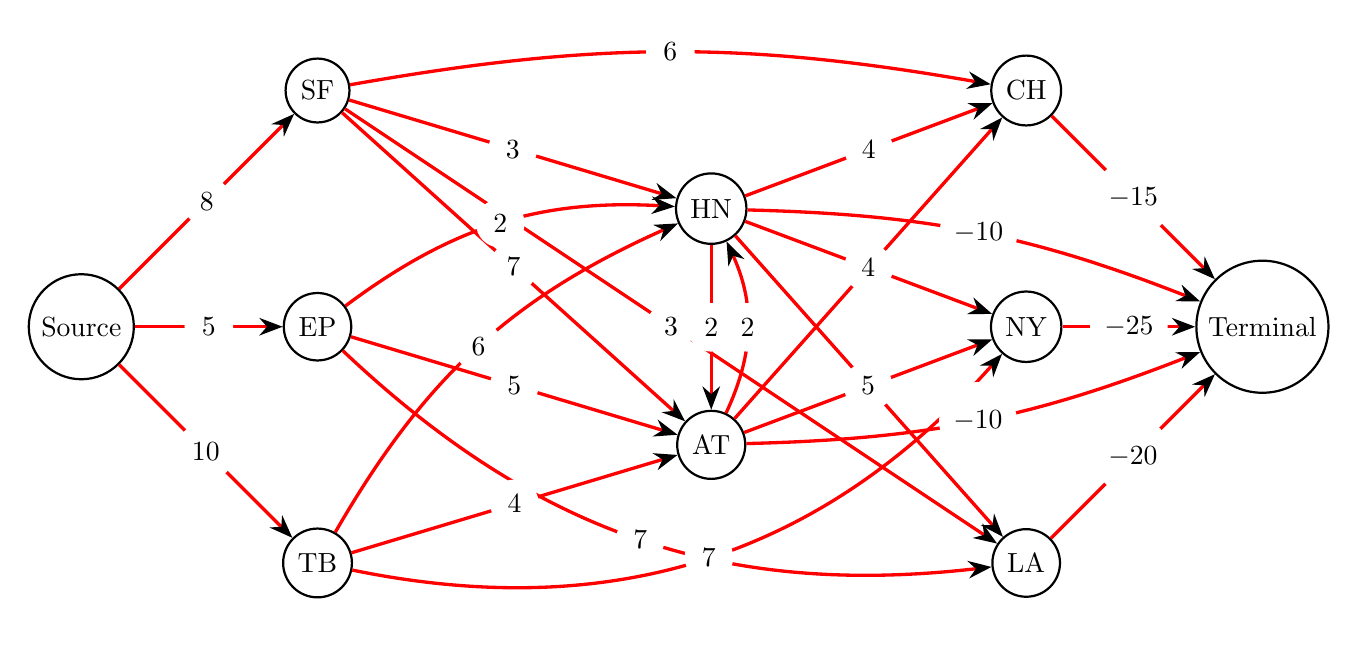
\begin{tikzpicture}
        \begin{scope}[every node/.style = {circle, thick, draw}]
            \node (A) at (0, 1)   {Source};

            \node (B) at (3, 4)   {SF};
            \node (C) at (3, 1)   {EP};
            \node (D) at (3,-2)   {TB};

            \node (E) at (8,  2.5)   {HN};
            \node (F) at (8, -0.5)   {AT};

            \node (G) at (12, 4)  {CH};
            \node (H) at (12, 1)  {NY};
            \node (I) at (12,-2)  {LA};

            \node (J) at (15, 1)  {Terminal};
        \end{scope}

        \begin{scope}[>={Stealth[black]},
                        every node/.style={fill=white,circle},
                        every edge/.style={draw=red,very thick}]
            \path [->] (A) edge node {$8$} (B);
            \path [->] (A) edge node {$5$} (C);
            \path [->] (A) edge node {$10$} (D);

            \path [->] (B) edge[bend left=10] node {$6$} (G);
            \path [->] (B) edge node {$3$} (I);
            \path [->] (B) edge node {$3$} (E);
            \path [->] (B) edge node {$7$} (F);

            \path [->] (C) edge[bend left=20] node {$2$} (E);
            \path [->] (C) edge[bend right=25] node {$7$} (I);
            \path [->] (C) edge node {$5$} (F);

            \path [->] (D) edge[bend right=30] node {$7$} (H);
            \path [->] (D) edge[bend left=18] node {$6$} (E);
            \path [->] (D) edge node {$4$} (F);

            \path [->] (E) edge node {$4$} (G);
            \path [->] (E) edge node {$5$} (I);
            \path [->] (E) edge node {$6$} (H);
            \path [->] (E) edge node {$2$} (F);
            \path [->] (E) edge[bend left=10] node {$-10$} (J);
            
            \path [->] (F) edge node {$4$} (G);
            \path [->] (F) edge node {$5$} (H);
            \path [->] (F) edge[bend right=25] node {$2$} (E);
            \path [->] (F) edge[bend right=10] node {$-10$} (J);

            \path [->] (G) edge node {$-15$} (J);
            \path [->] (H) edge node {$-25$} (J);
            \path [->] (I) edge node {$-20$} (J);

        \end{scope}
    \end{tikzpicture}

    We can see now that our program looks a little bit different, with our
    objective function no longer having any zeros as it did before. Another
    value we will want to change is actually withing our \texttt{b} vector,
    where we want to change the value associated with the demand of each node.
    Previously we had the deman of EP, SF, and TB as being negative values, but
    now we will make them zero. This is because, in order for a price to be
    associated with the production of the ducks, we need to have them traverse
    the edges connected to the source node. So now, we give the source node a
    demand of -1100. The Terminal node value we can keep the same, as it
    will still only get the number of ducks entered into the system.

    It is worth noting, that technically we could set the -1100 value to
    anything, but, considering the demand of our cities is exactly 1100 ducks,
    sending any more than 1100 ducks would reusult in a higher cost as those
    ducks wouldn't actuall by sold.

    \newpage

    With all of these factors in mind, we get a linear program that looks like
    the following...

    \begin{lstlisting}[style=mystyle, gobble=8]
        c_prof = np.array([10, 5, 8, 7, 4, 6, 5, 2, 7, 7, 3, 3, 6, 5, -10, 
                           4, 2, 2, 6, 4, -10, 5, -25, -15, -20])
        b_prof = np.array([-1100, 0, 0, 0, 150, 300, 250, 200, 200, 0])
        
        res_prof = linprog((-1) * c_prof, A_eq = A, b_eq = b_prof, A_ub = Aub, b_ub = bub)
    \end{lstlisting}
    Note, we are running this program with the same values for the A matrix, as
    the overal conservation of the nodes should remain the same. We are also
    running it with the same \texttt{bub} as that should not change for this
    problem either.
    This gives us the following results:

    \begin{minipage}[t]{.42\linewidth}
        \begin{lstlisting}[basicstyle=\small, gobble=12]
            fun:
             -18249.999931370083
            e_0  	 S/TB 	----> 600
            e_1  	 S/EP 	----> 100
            e_2  	 S/SF 	----> 400
            e_3  	 TB/NY 	----> 200
            e_4  	 TB/AT 	----> 200
            e_5  	 TB/HN 	----> 200
            e_6  	 EP/AT 	----> 100
            e_7  	 EP/HN 	----> 0
            e_8  	 EP/LA 	----> 0
            e_9  	 SF/AT 	----> 200
            e_10  	 SF/HN 	----> 200
            e_11  	 SF/LA 	----> 0
            e_12  	 SF/CH 	----> 0
            e_13  	 AT/NY 	----> 50
            e_14  	 AT/T 	----> 0
            e_15  	 AT/CH 	----> 200
            e_16  	 AT/HN 	----> 200
            e_17  	 HN/AT 	----> 100
            e_18  	 HN/NY 	----> 0
            e_19  	 HN/CH 	----> 0
            e_20  	 HN/T 	----> 0
            e_21  	 HN/LA 	----> 200
            e_22  	 NY/T 	----> 0
            e_23  	 CH/T 	----> 0
            e_24  	 LA/T 	----> 0
        \end{lstlisting}
    \end{minipage} \hfill \vline \hfill %
    \begin{minipage}[t]{.42\linewidth}
        So, there are many things to note about this output, the most important
        of which, is that it is almost certainly completely incorrect. We can
        notice that the edges leading to the terminal nodes have \textit{no
        ducks traversing them}. This is an immediate red flag, as our program
        relies on ducks traversing this in order to actually produce a profit.
        I tried many different things to get this to work, including changing
        values for the matrices involved, but I couldn't get the program to
        work as hoped. We can see, however, that ducks do in fact traverse the
        source node edges, which is as expected. 

        \medskip

        We can also note the negative function value. This, I though, was good
        at first, before I realized that I was actually maximizing this problem
        as seen by the negative one. So a negative value means something else
        is going wrong here, or at least, certainly a negative value of this
        magnitude is indicative of something going wrong here.
    \end{minipage}

    If we look at the production of various cities changes as compared to the
    previous examples. Namely TB produces less, as with EP, but SF produces
    more than previous examples.

    So, unfortunately this part of the problem was a bit of a failure, but
    hopefully I can bug fix it in the future, because I really do want to know
    what this problem would result in!

    As a side note, thank you so much for letting me take some extra time. I
    was able to sleep a little easier (not terribly well however) knowing that
    I had a little extra time to finish the report.
    \medskip
    \begin{center}
        \textit{fin}
    \end{center}

\end{document}
